\chapter{Aplicaciones continuas}%
\label{cha:aplicaciones_continuas}
En general en Matemáticas, cuando se estudia una estructura y sus propiedades, el paso inmediatamente posterior es estudiar los morfismos (las transformaciones) entre estas estructuras. En nuestro caso, el estudio de las aplicaciones entre espacios topológicos estará fundamentado en una característica clave, no sólo para el Análisis, sino también para la Topología: la continuidad.

A partir de este capítulo, vamos a estudiar las buenas propiedades que adquieren las aplicaciones continuas por la forma en que transforman los abiertos entre espacios y relacionan las topologías de cada uno.

\section{Definición de continuidad}%
\label{sec:continuidad}

Si hacemos memoria, recordaremos la famosa definición $\varepsilon-\delta$ para la continuidad que nos dieron para $\left( \mathbb{R}^n, \mathcal{T}_u \right)$. Esta venía decir que una función $f : X \rightarrow Y$ era continua en un punto $x_0\in X$ si y sólo si:
\[
\forall \varepsilon > 0, \ \exists \delta > 0 : \left(\lVert x - x_0 \rVert < \delta \Rightarrow \lVert f(x) - f(x_0) \rVert \right)
\]
y podemos reescribir esto último como $x \in B\left( x_0, \delta \right) \Rightarrow f\left( x \right) \in B\left( f\left( x_0 \right), \varepsilon \right)$ o también como $f\left( B\left( x_0, \delta \right) \right) \subset B\left( f\left( x_0 \right), \varepsilon \right) $. Lo anterior sugiere que la definición más ajena a las propiedades métricas y topológicas de $\mathbb{R}^n$ sería:
\[
\forall B\left( f\left( x_0 \right), \varepsilon \right),\ \exists B\left( x_0, \delta \right) \subset f^{-1}\left( B\left( f\left( x_0 \right), \varepsilon \right) \right)
\]
Sin embargo, esta definición sólo es válida para los espacios con la topología usual, pues el concepto de bola puede ser (y significar) cosas muy distintas en función de la topología empleada (sin ir más lejos puede no ser un abierto). Por ello, la siguiente definición pretende desligar el concepto de continuidad de la topología usual de $\mathbb{R}^n$ para que pueda ser aplicable a cualquier espacio topológico.

\begin{defi}[Continuidad]
Sean $X$ e $Y$ dos espacios topológicos y $f: X \rightarrow Y$ una aplicación entre ambos, decimos que $f$ es \textbf{continua en $x_0$ $\in X$} si y sólo si:
\[
\forall V^{f\left( x_0 \right)} :  f^{-1}\left( V^{f\left( x_0 \right)} \right) = V^{x_0} 
\]
es decir, la preimagen de cualquier entorno de $f(x_0)$ es entorno de $x_0$.
\end{defi}

\begin{prop}[Composición de continuidades]
Sean $f:X \rightarrow Y$ y $g: Y \rightarrow Z$ funciones continuas en $x_0\in X$ e $y_0\in Y$ tales que $f(x_0) = y_0$, la composición $h = g \circ f$ es una función continua en $x_0$.
\end{prop}
\begin{demo}
Escojamos un entorno $V^{h\left( x_0 \right)}$ de la imagen por $h$ de $x_0$, entonces
\[
h^{-1} V^{h\left( x_0 \right)} = f^{-1}g^{-1}V^{g\left( y_0 \right)} = f^{-1} V^{y_0} = V^{x_0}
\]
\end{demo}

\begin{ej}
\begin{enumerate}
    \item Sea $f: X_{\text{discreta}} \rightarrow Y$, entonces es continua sean cuales sean los conjuntos de partida y de llegada, pues todo es abierto y, en consecuencia, todo es entorno en $\mathcal{T}_{\text{disc}}$.
    \item Sea $f: X \rightarrow Y_{\text{trivial}}$, entonces es continua sean cuales sean los conjuntos de partida y de llegada, pues como $Y$ es el único abierto, entonces es el único entorno $V^{f\left( x \right)}$ para cualquier $f(x)$ y $f^{-1}V^{f\left( x \right)} = f^{-1}Y = X$, que es abierto.
    \item Si una función $f: X \rightarrow Y_{\text{discreta}}$ es continua, entonces $f$ es localmente constante, pues como en la trivial los puntos son abiertos, entonces el punto $\{f\left( x_0 \right)\}$ es entorno $V^{f\left( x_0 \right)}$ de sí mismo. Por tanto, por la continuidad de $f$, $f^{-1}f\left( x_0 \right) = V^{x_0}$, luego $f \equiv f\left( x_0 \right)$ en ese entorno $V^{x_0}$.
    \item Si una función $f: X \rightarrow Y$ es localmente constante, entonces es continua, puesto que si es localmente constante para cualquier $x_0 \in X$ existe un entorno $U^{x_0} : f\mid_{U^{x_0}} \equiv f\left( x_0 \right)$. De este modo, cualquier entorno $V^{f\left( x_0 \right)}$ de la imagen $f(x_0)$ cumple que $f^{-1}V^{f\left( x_0 \right)} \supset U^{x_0}$ y llamando $V^{x_0} = f^{-1} V^{f\left( x_0 \right)}$ entonces vemos que es entorno de $x_0$.
\end{enumerate}
\end{ej}

\begin{prop}[Caracterización de Continuidad]
Sea $f:X\rightarrow Y$ una función entre espacios topológicos, entonces son equivalentes:
\begin{enumerate}
    \item $f$ es continua.
    \item $\forall U \ab Y : f^{-1}\left( U \right) \ab X$.
    \item $\forall F \cerr Y : f^{-1}\left( F \right) \cerr X$.
    \item $\forall A \subset Y : f^{-1}\left( \mathring{A} \right) \subset \inter\left( f^{-1}\left( A \right) \right)$.
    \item $\forall A \subset X : f\left( \overline{A} \right) \subset \overline{f\left( A \right)}$.
\end{enumerate}
\end{prop}
\begin{demo}
\begin{itemize}
    \item $1. \Rightarrow 2.$
    
    Escojamos un abierto cualquiera $W \ab Y$. Por ser abierto, es entorno de todos sus puntos y, en particular, es entorno de las imágenes que puedan caer dentro de dicho abierto, es decir, $\forall x \in f^{-1} (W) : W = V^{f(x)}$. Por continuidad, las preimágenes de entornos de las imágenes son entornos de las preimágenes, luego $\forall x \in f^{-1} W : f^{-1}W = V^x$ y, como es entorno de todos sus puntos, entonces $f^{-1} W \ab X$.
    \item $2. \Rightarrow 3.$
    
    Como lo que sabemos es que las preimágenes de abiertos son abiertas y los cerrados se definen en términos de abiertos, no nos queda otra estrategia que intentar demostrarlo pasando los cerrados a sus complementarios: los abiertos.
    
    Escojamos un cerrado cualquiera $C \cerr Y$ de modo que conocemos que $Y \setminus C \ab Y$. Como conocemos el resultado para abiertos, podemos decir que $f^{-1}\left( Y\setminus C \right) \ab X$ y, conjuntistamente, $X \setminus f^{-1}C = f^{-1}\left( Y\setminus C \right)$, luego directamente tenemos que $f^{-1}C \cerr X$. 
    \item $3. \Rightarrow 5.$
    
    Como $\overline{f\left( A \right)} \cerr Y$ sabemos que $f^{-1}\overline{f\left( A \right)} \cerr X$. Como $A\subset f^{-1}f(A) \subset f^{-1}\overline{f\left( A \right)}$ y este último es cerrado en $X$, entonces $\overline{A}\subset f^{-1}\overline{f\left( A \right)}$ y, por tanto, $f\left( \overline{A} \right) \subset \overline{f\left( A \right)}$.
    \item $5. \Rightarrow 4.$
    \begin{gather*}
        Y \setminus \mathring{A}\Rightarrow \overline{Y\setminus A} \supset \overline{f\left( X \setminus f^{-1}A \right)} \stackrel{5)}{\supset} f\left( \overline{X \setminus f^{-1}\left( A \right)} \right) = f\left( X \setminus \inter\left( f^{-1}A \right) \right) \Rightarrow\\
        X \setminus \inter\left( f^{-1}A \right) \subset f^{-1}\left( Y\setminus \mathring{A} \right) = X \setminus f^{-1}\left( \mathring{A} \right)\Rightarrow f^{-1}\left( \mathring{A} \right) \subset \inter\left( f^{-1}A \right) 
    .\end{gather*}

    \item $4 \Rightarrow 1)$
    \begin{gather*}
        V^{f\left( x \right)} \Rightarrow f\left( x \right) \in \inter\left( V^{f\left( x \right)} \right) \Rightarrow x \in f^{-1}\left( \inter\left( V^{f\left( x \right)} \right) \right) \subset \inter\left( f^{-1}V^{f\left( x \right)} \right) \Rightarrow \\
        f^{-1}V^{f\left( x \right) } \text{ entorno de } x.
    \end{gather*}
\end{itemize}
\end{demo}

\begin{obs}
La definición y posterior caracterización nos permiten recuperar las propiedades de continuidad a las que estamos habituados, como por ejemplo el quinto apartado del que se desprende que la imagen del límite es el límite de la imagen, pero también nos da la posibilidad de utilizar dicha continuidad con fines meramente topológicos, como por ejemplo $id: \left( X, \mathcal{T}_1 \right) \rightarrow \left( X, \mathcal{T}_2 \right)$ es continua si y sólo si $\mathcal{T}_2 \subset \mathcal{T}_1$ (por 1).
\end{obs}

\section{Continuidad y subespacios}%
\label{sec:continuidad_y_subespacios}
En muchas ocasiones tiene interés estudiar el comportamiento de una función, no en el conjunto total, sino en un subconjunto de puntos concreto. Como hemos definido anteriormente los subespacios topológicos, tiene sentido querer ver cómo se comportan las aplicaciones y sobre todo la continuidad, cuando trabajamos con estos subconjuntos.

\begin{prop}
Sea $f: X \rightarrow Y$ una función continua y $Z \subset X$ un subespacio topológico, entonces la restricción $f|_Z : Z \rightarrow Y$ también es continua.
\end{prop}
\begin{demo}
Aplicando la caracterización de continuidad a través de las preimágenes de abiertos, tenemos que:
\[
\forall A \ab Y : \left( f|_Z \right)^{-1} \left( A \right) = Z \cap f^{-1} A \ab Z
\]
donde este último conjunto es abierto por la definición de topología relativa.
\end{demo}

%TODO: Diagramas composición
\begin{obs}
\begin{enumerate}
    \item La aplicación inclusión $Z \stackrel{j}{\subset} X$ es continua.
    \begin{demo}
     Para cualquier abierto $U \ab X$ la preimagen $j^{-1}\left( U \right)$ corresponde a los puntos de $U \cap Z$, y este último conjunto es abierto en $Z$ por definición.
    \end{demo}

    \item La continuidad se hereda en la restricción a un subespacio, es decir, si consideramos la aplicación $Z \stackrel{j}{\subset} X \xrightarrow{f} Y$, entonces la continuidad de $f$ implica\footnote{Pero el recíproco no es cierto, la continuidad en un subespacio no extiende la continuidad a todo el espacio.} la continuidad de $f|_Z$.
    \begin{demo}
    Como $f|_Z = f \circ j$ y ambas son continuas, por composición, $f|_Z$ es continua.
    \end{demo}

    \item La continuidad es una propiedad local, es decir, que si $f|_{E^x}$ continua en $x$, entonces $f$ continua en $x$.
    \begin{demo}
	La preimagen de cualquier entorno $V^{f\left( x \right)}$ es $\left( f|_{E} \right)^{-1} \left( V^{f\left( x \right)} \right) = W^x$ un entorno de $x$ en $E^x$, pero tenemos que ver que lo es en $X$ para poder afirmar que es continua.
	Como $W^x \stackrel{\text{ent.}}{\subset} E^x \stackrel{\text{ent.}}{\subset} X$, entonces $W^x \stackrel{\text{ent.}}{\subset}X$, ya que entorno de entorno es entorno.
	
	Esta última afirmación es cierta porque:
        \begin{gather*}
        \begin{rcases}
           	W^x \stackrel{\text{ent.}}{\subset} E^x \Rightarrow \exists G \ab E^x \mbox{ tal que }G \subset W^x, \ G = A \cap E^x \subset X\\ 
            E^x \stackrel{\text{ent.}}{\subset} X \Rightarrow \exists B \ab X \mbox{ tal que } B \subset E^x
        \end{rcases}\Rightarrow\\
        x \in \underbrace{A \cap B}_{\ab X} \subset \underbrace{A \cap E^x}_{= G}  \subset W^x
        \end{gather*}
    \end{demo}

    \item Si $f|_{U \ab X}$ es continua $\Rightarrow f$ continua $\forall x \in U$.

    \item $x$ es aislado $\Rightarrow f$ continua en $x$. 
    \begin{demo}
        $x$ aislado $\Leftrightarrow V^x = \{x\}$ es abierto de $X$. $f|_{V^x} : \{x\} \rightarrow Y$.
    \end{demo}

    \item $f: X \rightarrow Y \supset Z$ tal que $f\left( X \right) \subset Z \subset Y$ (si no es así puede estar mal definido).

    Entonces, $f$ a $Y$ es continua $\Leftrightarrow f$ a $Z$ es continua.
    \begin{demo}
        \begin{itemize}
            \item $f$ cont. en $Z \xRightarrow{j \circ f} f$ cont. en $Y$. %TODO: Seguro?
            \item $f$ cont. en $Y \xRightarrow{?} f$ cont. en $Z$. 

            Sea $U_z$ ab. en $Z$. Este será $U_y \cap Z = U_z$ que cumple, $f_z^{-1}\left( U_y \cap Z \right) \stackrel{f\left( X \right) \subset Z}{=}  f_y^{-1}\left( U_y \right)$ que es abierto en $X$ (por ser $f_y$ continua).
        \end{itemize}
    \end{demo}
\end{enumerate}
\end{obs}

\begin{prop}[Criterios de continuidad por recubrimientos]
Sea $f: X \rightarrow Y$ una función entre espacios topológicos, si se da alguna de las siguientes condiciones: 
\begin{align*}
\begin{cases}
X = \bigcup_{i \in  I} U_i \mbox{ donde } U_i \ab X \\
\forall f|_{U_i} : U_i \rightarrow Y \mbox{ cont.}
\end{cases}
& &
\begin{cases}
X = \bigcup_{i =0}^n F_i \mbox{ donde } F_i \cerr X \\
\forall f|_{F_i} : F_i \rightarrow Y \mbox{ cont.}
\end{cases}
\end{align*}
entonces la función $f$ del inicio es continua.
\end{prop}
\begin{demo}
	\begin{itemize}
	\item Escojamos un abierto cualquiera $W \ab Y$ y veamos si su preimagen $f^{-1}W$ es un abierto en $X$.

    En primer lugar, por ser $X = \bigcup_{i \in  I} U_i$ podemos escribir que $f^{-1}W = X\cap f^{-1}W = \bigcup_{i \in  I} U_i \cap f^{-1} W = \bigcup_{i \in  I} \left( U_i \cap f^{-1} W\right) = \bigcup_{i \in  I} \left( f|_{U_i} \right)^{-1} W$. Como $\left( f|_{U_i} \right)^{-1}W \stackrel[\text{(cont.)}]{\text{ab.}}{\subset} U_i \ab X$, entonces $\left( f|_{U_i} \right)^{-1} W \ab X$ y de esta manera podemos escribir $f^{-1}W$ como unión de abiertos $\bigcup_{i \in  I} \left( f|_{U_i} \right)^{-1} W$ de $X$, es decir, que $f^{-1}W \ab X$.
	
	\item Escojamos un cerrado cualquiera $C \cerr Y$ y veamos si su preimagen $f^{-1}C$ es cerrada en $X$.

    En primer lugar, por ser $X = \bigcup_{i=0}^n F_i$ podemos escribir que $f^{-1}C = X\cap f^{-1}C = \bigcup_{i = 0}^n F_i \cap f^{-1} C = \bigcup_{i = 0}^n \left( F_i \cap f^{-1} C\right) = \bigcup_{i = 0}^n \left( f|_{F_i} \right)^{-1} C$. Como $\left( f|_{F_i} \right)^{-1}C \stackrel[\text{(cont.)}]{\text{cerr.}}{\subset} F_i \cerr X$, entonces $\left( f|_{U_i} \right)^{-1} C \cerr X$ y de esta manera podemos escribir $f^{-1}C$ como unión finita de cerrados $\bigcup_{i = 0}^n \left( f|_{F_i} \right)^{-1} C$ de $X$, es decir, que $f^{-1}C \cerr X$.
    \end{itemize}
\end{demo}


\section{Homeomorfismos}%
\label{sec:homeomorfismos}
Supongamos que tenemos una función $f$ biyectiva y continua. Con las definiciones de continuidad anteriores hemos caracterizado la topología de las imágenes por $f^{-1}$, pero no sabemos nada de cómo se comporta la función $f$ con respecto a abiertos, cerrados, etc.
Nos gustaría poder destacar en qué condiciones una función establece una biyección entre abiertos de dos espacios, pues de esa forma existiría un ``isomorfismo'' entre ambas topologías a la hora de trabajar con ellas. 

\begin{defi}[Aplicaciones abiertas y cerradas]
Sea $f: X \rightarrow Y$ una función entre espacios topológicos, decimos que es:
\begin{itemize}
\item \textbf{abierta} si y sólo si las imágenes de abiertos son abiertos.
\item \textbf{cerrada} si y sólo si las imágenes de cerrados son cerrados.
\end{itemize}
\end{defi}

\begin{obs}
La caracterización que dimos de la continuidad hacía referencia a las preimágenes de abiertos y cerrados, no a sus imágenes. De hecho, ni la continuidad implica que la aplicación sea abierta o cerrada, ni viceversa.
\end{obs}

\begin{ej}
En la siguiente tabla podemos ver distintos ejemplos de funciones que verifican algunas de las condiciones que hemos definido, pero no otras simultáneamente:
\begin{table}[H]
\centering
\begin{tabular}{c|c|c|c}
Función & continua & abierta & cerrada \\
\hline
$Id: X_{\text{trivial}} \rightarrow X_{\text{discreta}}$ & \ding{55} & \checkmark & \checkmark \\
\hline
$Id: X_{\text{discreta}} \rightarrow X_{\text{trivial}}$ & \checkmark & \ding{55} & \ding{55} \\
\hline
$j: \left[ 0, 1 \right] \subset \mathbb{R}_{u}$ & \checkmark & \ding{55} & \checkmark \\
\hline
$j: \left( 0, 1 \right) \subset \mathbb{R}_u$ & \checkmark & \checkmark & \ding{55} \\
\hline
\end{tabular}
\caption{\textit{En la tabla anterior podemos ver ejemplos de funciones que son continuas, abiertas o cerradas de distintas formas.}}
\end{table}
\end{ej}

\begin{prop}[Trivialidades esenciales]
Sea $f:X\rightarrow Y$ una función biyectiva, entonces las siguientes afirmaciones:
\begin{enumerate}
    \item $f$ es abierta
    \item $f$ es cerrada
    \item $f^{-1}$ es continua.
\end{enumerate}
son equivalentes.
\end{prop}
\begin{demo}
\begin{itemize}
    \item $1. \Rightarrow 2.$
    
    Sea $F \cerr X$, por la definición de cerrado su complementario $X\setminus F$ es abierto en $X$. De esta manera, como $f$ es abierta, entonces $f\left( X\setminus F \right) \ab X$. Por la biyectividad, $f\left( X\setminus F \right) = Y\setminus f\left( F \right)$, es decir, que $f\left( F \right) \cerr Y$, lo que demuestra que $f$ es cerrada.

    \item $2. \Rightarrow 3.$
    
    Sea $F \cerr X$, como $f$ es cerrada, $f\left( F \right) \cerr Y$. Pero $f(F)= \left( f^{-1} \right)^{-1} \left( F \right)$ por la biyectividad de $f$, luego hemos demostrado que $f^{-1}$ continua porque las preimágenes de cerrados son cerrados.

    \item $3. \Rightarrow 1.$
    
    Sea $U \ab X$, por la continuidad de $f^{-1}$, la preimagen $\left( f^{-1} \right)^{-1} \left( U \right) \ab Y$. Por tanto, como $f\left( U \right) =  \left( f^{-1} \right)^{-1} \left( U \right)$, hemos demostrado que $f$ es abierta.
\end{itemize}
\end{demo}

\begin{defi}[Homeomorfismo]
Sea $f: X \rightarrow Y$ una aplicación biyectiva, decimos que es un \textbf{homeomorfismo} si y sólo si $f$ y $f^{-1}$ son continuas o, equivalentemente, si $f$ es continua y abierta o cerrada.
\end{defi}

\begin{obs}
La definición de homeomorfismo es importante porque no establece simples biyecciones entre conjuntos, establece biyecciones sobre topologías:
\begin{align*}
	f: \mathcal{T}_X &\rightarrow \mathcal{T}_Y\\
	U &\mapsto f\left( U \right)\\
	f^{-1}\left( W \right) &\mapsfrom W 
\end{align*}
lo que permite trabajar con los abiertos de un lado y trasladar el mismo trabajo a los del otro de forma canónica.
\end{obs}

\begin{defi}[Homeomorfismo Local]
Sea $f: X \rightarrow Y$ una función entre espacios topológicos, decimos que es un \textbf{homeomorfismo local en $x_0 \in X$} si y sólo si existen algunos entornos $V^{x_0}$ y $V^{f\left( x_0 \right)}$ tales que la restricción $f: V^{x_0} \rightarrow V^{f\left( x_0 \right)}$ es un homeomorfismo.
\end{defi}

\begin{obs}
En general, cuando decimos que una aplicación $f:X\rightarrow Y$ es un homeomorfismo local sin especificar en qué punto, estamos diciendo que es homeomorfismo local para cualquier punto $x\in X$.

Además, en la definición de homeomorfismo local anterior, podemos tomar $V^{x_0}$ y $V^{f\left( x_0 \right)}$ como entornos abiertos.
%TODO: Habría que meter un diagrama de flechas como el que hizo en clase (preguntar a JD por él si no lo encontramos)
\begin{demo}
Si $f$ es homeomorfismo local, entonces $\exists V^a \subset X$ y $V^{f\left( a \right)} \subset Y$ tal que $f: V^a \rightarrow V^{f\left( a \right)}$ es homeomorfismo y, por esta razón, sabemos que $\exists U^a \ab V^a$ tal que $f\left( U^a \right) \ab V^{f\left( a \right)}$. 

Además, como $f(U^a)$ es abierto en $V^{f\left( a \right)}$, sabemos que $f(U^a)$ es entorno\footnote{En este punto no podemos parar y decir que es abierto porque lo que sabemos es que $f(U^a)$ es abierto en $V^{f(a)}$, pero no sabemos nada sobre si es abierto en $Y$, que es lo que necesitamos.} de $f(a)$ en $V^{f(a)}$. Como tenemos la secuencia $f(U^a) \ent V^{f(a)} \ent Y$, sabemos que $f(U^a) \ent Y$ de $f(a)$ y, por tanto, podemos encontrar un abierto $W \ab Y$ tal que $W\subset f(U^a)$.

Por tanto, como se trata de un homeomorfismo local, existirá algún $G \ab U^a$ de forma que $f(G) = W$. Pero como $U^a$ es abierto global, entonces tenemos que $G\ab X$ y hemos acabado, pues tenemos el homeomorfismo local definido en $f: G \rightarrow W$.
\end{demo}
\end{obs}

\begin{prop}[Conservación por restricción]
Sea $f: X \rightarrow Y$ un homeomorfismo, la restricción $f: Z \rightarrow f\left( Z \right)$ a cualquier subespacio $Z \subset X$ también es homeomorfismo.
\end{prop}
\begin{demo}
La restricción será biyectiva por serlo $f$ y ser el conjunto de llegada $f(Z)$. Una biyección es homeomorfismo si tanto $f$ como $f^{-1}$ son continuas y como ya vimos que la restricción de una continua es continua, sabemos que la restricción de $f$ y $f^{-1}$ a $Z$ y $f\left( Z \right)$ son también continuas, es decir, $f|_Z$ es homeomorfismo.
\end{demo}

\begin{prop}[Conservación por composición]
Sean $f: X \rightarrow Y$ y $g: Y \rightarrow Z$ dos homeomorfismos, su composición $h = f \circ g$ también es homeomorfismo.
\end{prop}

\begin{prop}
Sea $f:X\rightarrow Y$ un homeomorfismo local, entonces es abierto.
\end{prop}
\begin{demo}
Hay dos formas de demostrarlo, la primera es intentando ver que para cualquier $U \ab X$ ocurre que $f\left( U \right)$ es entorno de las imágenes de todos los puntos de $U$.

Con este objetivo, sabemos que por ser $f$ homeomorfismo local existe una restricción $\exists f| : V^{x_0} \rightarrow V^{y_0}$ para cada punto $x_0\in U$ y usando la notación $y_0 = f(x_0)$. Como esta restricción es homeomorfismo, $f\left( U \cap V^{x_0} \right) \ab V^{y_0}$ y, por tanto, $ f \left( U \cap V^{x_0} \right)$ es entorno en $Y$ de $y_0$. Al ocurrir esto para todos los puntos y, teniendo en cuenta que $f \left( U \cap V^{x_0} \right)\subset f(U)$, sabemos que $f(U)$ es entorno de las imágenes de todos los puntos de $U$.

La otra forma de verlo es que, por ser homeomorfismo local, para cualquier punto $x\in X$ existe un entorno abierto $W^x \ab X$ de forma que $f(W^x)\ab Y$ es abierto. De esta manera, y abusando de la notación, escribiendo $W^x = W^x \cap U$, $U$ puede expresarse como $U = \bigcup_{x\in U} W^x$. Por tanto, $f(U) = f(\bigcup_{x\in U} W^x) = \bigcup_{x\in U} f(W^x)$ que es unión de abiertos, luego es abierto.
\end{demo}

% TODO: estos ejemplos hay que mirarlos despacio y corregirlos
\begin{ej}[¡Importantes!]
\begin{enumerate}
    \item \textbf{Proyección estereográfica}:

    Sea $\mathbb{S}^m$ y $a \in \mathbb{S}^m \Rightarrow \mathbb{S}^{m} \setminus \{a\} \rightarrow \mathbb{R}^m$ homeomorfismo. ($\mathbb{R}^{m}$ es en realidad un hiperplano de $\mathbb{R}^{m+1}$ en el que se encuentra contenida la ``esfera'')

    \item \textbf{Proyección exponencial}: 

    $\mathbb{R} \rightarrow \mathbb{S}^1: \theta \mapsto e^{2\pi i\theta} = \left( \cos 2\pi \theta, \sin 2\pi \theta \right)$ es homeomorfismo local, pero no es inyectiva al ser periódica.

    \item \textbf{Proyección antipodal}:

    $\mathbb{R}^{m+1}\setminus \{0\} \supset \mathbb{S}^m \rightarrow \mathbb{R}\mathrm{P}^{m}: x \mapsto \left[ x \right]$ es homeomorfismo local. Es 2-1 por llevar las antípodas al mismo $\left[ x \right]$. 

    Podemos dividir $\mathbb{S}^{m}$ tal que: $\mathbb{S}^{m} = S_{+} \cup S_{-} \cup E$ (ecuador). Llamando $U_p$ a todas las rectas no contenidas en el plano ortogonal a la recta formada por el punto que se quita y su antípoda. Con esto tenemos $U_p \simeq \mathbb{R}^{m}$. Uniéndolo con el hiperplano del infinito $H_p^{\infty}$ tenemos que los polos van a $U_p$ y $E$ a $H_p^{\infty}$. Esta correspondencia es homeomorfa por lo que se puede trasladar la topología.

    Con esto, esta proyección será un recubrimiento doble de $\mathbb{R}\mathrm{P}^m,\ m \ge 2$.

    \item \textbf{Lemniscata}:

    $f: \mathbb{R} \rightarrow X \subset \mathbb{R}^2: t \mapsto \left( \frac{t}{1 + t^4}, \frac{t^3}{1 + t^4} \right)$ es biyectiva y continua, pero NO homeomorfismo local.
    \begin{figure}[H]
        \centering
        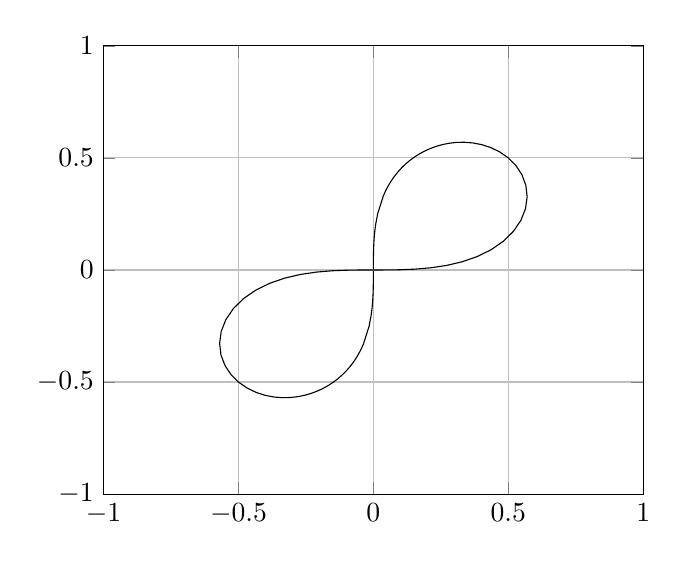
\begin{tikzpicture}
            \begin{axis}[
                xmin=-1,xmax=1,
                ymin=-1,ymax=1,
                grid=both,
                ]
                %TODO: Aumentar el tamaño para la versión final
                %Ponemos varios intervalos para minimizar las samples y, por tanto, el tiempo de compilación.
                \addplot [domain=-3:3,samples=100]({(x/(1+x^4))},{(x^3/(1+x^4))}); 
                \addplot [domain=-3:-50,samples=50]({(x/(1+x^4))},{(x^3/(1+x^4))}); 
                \addplot [domain=-50:-200,samples=50]({(x/(1+x^4))},{(x^3/(1+x^4))}); 
                \addplot [domain=3:50,samples=50]({(x/(1+x^4))},{(x^3/(1+x^4))}); 
                \addplot [domain=50:200,samples=50]({(x/(1+x^4))},{(x^3/(1+x^4))}); 
            \end{axis}
        \end{tikzpicture}
        \caption{\textit{Representación Lemniscata.}}
        \label{fig:lemniscata}
    \end{figure}

    Engañosamente: 
    \[
        \forall t \in \mathbb{R},\ \exists \left( t - \varepsilon, t + \varepsilon \right) = I_{\varepsilon}: f| : I_{\varepsilon} \rightarrow f\left( I_{\varepsilon} \right) 
    \]
    es homeomorfismo.

    En $t = 0,\ f\left( I_{\varepsilon} \right)$ NO es entorno de $f\left( 0 \right) = \left( 0, 0 \right)$, porque se tienen que tomar elementos de la rama ``vertical''.

    \item Las \textbf{coordenadas polares} $\left( 0, \rightarrow \right) \times \mathbb{R}^{} \rightarrow \mathbb{R}^{2},\ \left( r, \theta \right) \mapsto \left( r\cos \theta, r \sin \theta \right)$ son homeomorfismo local con $\theta_0 \in \left( \theta_0 - \pi, \theta_0 + \pi \right)$ hasta $\mathbb{R}^{2} \setminus L$ con $L$ la recta entre $O$ y $\theta_0$.
\end{enumerate} 
\end{ej}

\begin{defi}[Variedad Topológica]
Una \textbf{variedad topológica} de dimensión $m$ es un espacio localmente homeomorfo a $\mathbb{R}^m$, es decir, que cada punto tiene un entorno abierto homeomorfo a una bola\footnote{Luego, en el fondo, es homeomorfo a cualquier bola y, por ser éstas parte de una base de $\mathbb{R}^m$, es homeomorfo a todo $\mathbb{R}^m$.} $B\left( 0, \varepsilon \right) \subset \mathbb{R}^m$.
\end{defi}
\begin{ej}
Esferas, espacios proyectivos, toros...
\end{ej}

